\section{Arbeitspaket 3.2}

\subsection{Dynamic Resource Usage Tracking}

\begin{frame}{Dynamische Ressourcen Auslastung}
    \begin{block}{Dynamische Ressourcen Auslastung}
        Aktuelle Auslastung der Ressourcen einer Menge von Knoten.\\
        Wie hoch ist die Ressourcen Auslastung einer Anwendung?
    \end{block}
    \begin{itemize}
        \item Auslastung von Arbeitsspeicher und lokalen Speicher, pro Knoten
            oder NUMA-Domain.
        \item Lastmessung zwischen Zentralen Dateisystem und Compute-Node.
        \item Auf\"{u}hrung, nebenl\"{a}ufig zur Anwendung.
        \item Der Anwendungscode soll nicht ver\"{a}ndert werden.
    \end{itemize}
\end{frame}


\begin{frame}{perf}

    \begin{itemize}
        \item Events Subsystem im Linux-Kernel.
        \item Instrumentiert Hardware Performance Counter, tracepoints, KProbes,
            UProbes.
        \item geringer Overhead.
    \end{itemize}

\end{frame}

\begin{frame}{perf}

    \begin{figure}
        \centering
        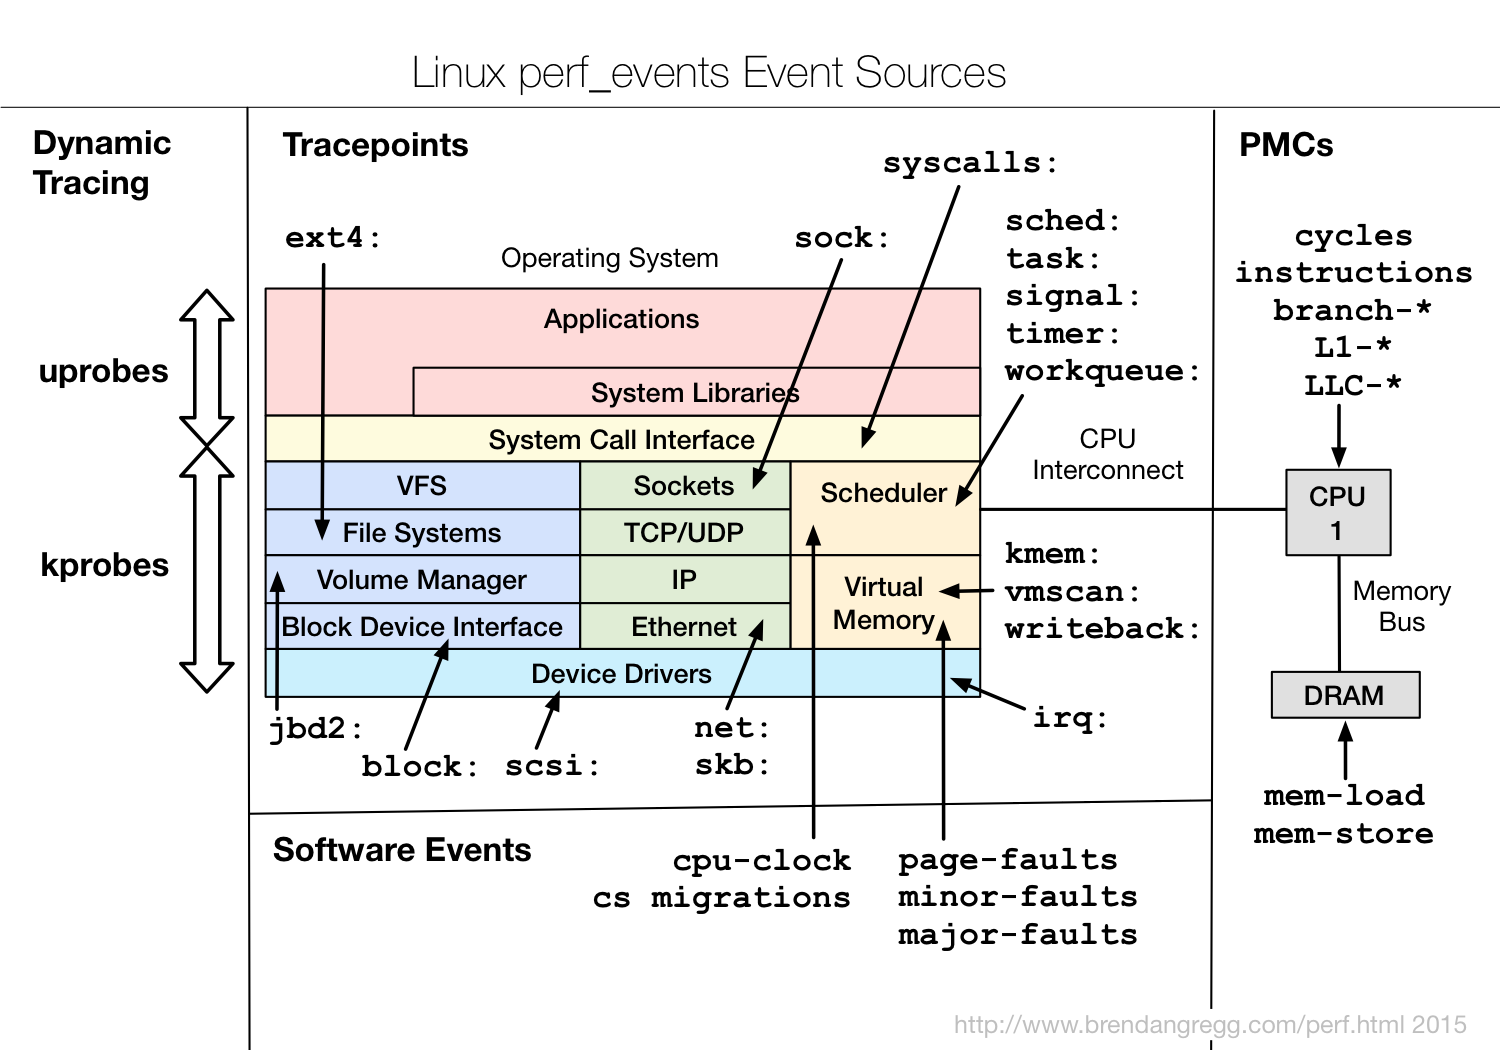
\includegraphics[width=0.79\textwidth]{fig/perf_events_map.png}
    \end{figure}
    \tiny{\href{perf}{http://www.brendangregg.com/perf\_events/perf\_events\_map.png}}
\end{frame}

\subsection{Integrated Monitoring}

\begin{frame}{Integrated Monitoring of the Ad-hoc File System}
    \begin{itemize}
        \item Integration der Monitoring Komponenten in das Ad-hoc Dateisystem.
        \item \"{U}berwachen von I/O Aufrufen an vier Schnittstellen.
            \begin{enumerate}
                \item Aufrufe von der Anwendung an das Dateisystem.
                \item Aufrufe des Ad-hoc Dateisystems zum unterliegenden Dateisystem.
                \item Anfragen vom \emph{data transfer executor}.
                \item Interner Datentransfer innerhalb des Ad-hoc Dateisystems.
            \end{enumerate}
        \item Aufgezeichnete I/O-Events werden in einer Datenbank gespeichert.
    \end{itemize}

    \begin{block}{Ziel}
        Analyse des Ad-hoc Dateisystems.
        Entwickelte Komponenten bieten Informationen zur Entwicklung und Optimierung des Systems.
    \end{block}
\end{frame}
